\chapter{Data Exploration and Visualization}
A Dataset is a collection of data, for instance a tabular representation of data which includes rows (istances-records-objects) and columns (attributes). It is important to note that the rows, or the samples are in the interval $1 \rightarrow M$, while the features are from $1 \rightarrow N$. 

The size of the Dataset has an impact on the choice of the analyses:
\begin{itemize}
    \item Some algorithms require considerable HW resources when applied to large datasets.
    \item There are solutions to reduce the size of the dataset preserving the completeness of the data:
    \begin{itemize}
        \item \textbf{Data Sampling:} reduce the dataset size in terms of number or rows, records ($m' < m$).
        \item \textbf{Feature Selection:} reduce the number of attributes, features ($n' < n$).
    \end{itemize}
\end{itemize}

Features (attributes), have a major role in the Dataset. Each column of the dataset represents on attribute.Data Exploration can use a univariate approach to analyze one column in isolation, or a multivariate approach to study the relationships and dependencies between multiple columns at the same time. 

For further analysis it's useful to consider basic information for each attribute such as the unite of measurement, attribute type (categorical or numerical) and the attribute domain, by also checking if the attribute values satisfy the domain-driven constraints.

\paragraph*{Notations}
\begin{itemize}
    \item $a \in \mathcal{A}$: Object $a$ is an element of the set $\mathcal{A}$.
    \item $|\mathcal{A}|$: The cardinality (number of elements) of a finite set $\mathcal{A}$.
    \item $\mathcal{A} \subseteq \mathcal{B}$: $\mathcal{A}$ is a subset of $\mathcal{B}$.
    \item $\mathcal{A} \subset \mathcal{B}$: $\mathcal{A}$ is a strict subset of $\mathcal{B}$.
    \item $\mathbb{N}$: The set of natural numbers $1, 2, \dots$.
    \item $\mathbb{R}$: The set of real numbers.
    \item $\{0, 1\}$: The set consisting of two real-numbers 0 and 1.
    \item $[0, 1]$: The closed interval of real numbers $x$ with $0 \le x \le 1$.
    \item $\mathbf{x} = (x_1, \dots, x_n)^T$: A vector of length $n$[cite: 2].
    \item $\|\mathbf{x}\|$: The norm of the vector $\mathbf{x}$ (usually the Euclidean norm).
\end{itemize}

\section{Univariate Analysis: Distribution}
When analyzing a single feature (a column in the dataset), we can treat the general concept it measures as an abstract \textbf{Random Variable ($X$)}. The actual data points we collected ($x_1, \dots, x_m$) are the concrete samples or realizations of that variable. 

Because we can never perfectly know the underlying mathematical law that generated this data (the \textbf{theoretical distribution}), we rely entirely on our collected samples to form an \textbf{empirical distribution} (An empirical distribution is the distribution formed by data values (denoted as $x_1, \dots, x_m$) that you have collected in your dataset.), which serves as our practical, real-world approximation. The most common way to visualize this empirical distribution is through a \textbf{histogram}: we slice the total range of our data into consecutive intervals called \textbf{bins}, and simply count how many data points fall into each bin (the \textbf{frequency}).

Probability Distributions are usually classified as:
\begin{itemize}
    \item \textbf{Discrete Probability Distribution:} discrete list of probabilities of outcomes and described by a probability mass function.
    \begin{figure}[h]
        \centering
        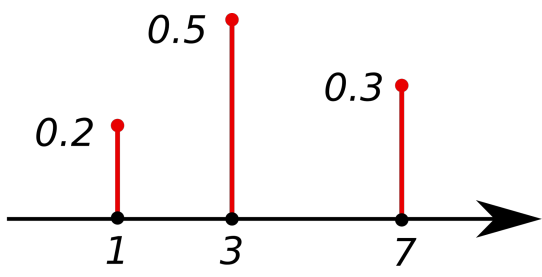
\includegraphics[width=0.3\linewidth]{images/chapter_2/PMF.png}
        \caption{Example of a Probability Mass Function (PMF)}
    \end{figure}
    
    \item \textbf{Continuous Probability Distribution:} set of possible outcomes can assume values in a continuous range and described by a probability density function.
    \begin{figure}[h]
        \centering
        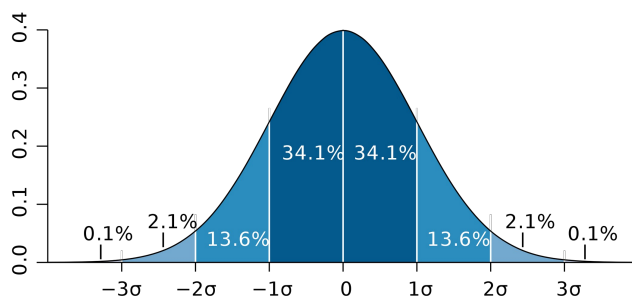
\includegraphics[width=0.3\linewidth]{images/chapter_2/PDF.png}
        \caption{Example of the Probability Density Function (PDF) of the normal distribution}
    \end{figure}
\end{itemize}

\subsection{Discrete and Continuous Probability Recall}
The Probability Mass Function present some limitations:

\begin{itemize}
    \item In cases of a lot of samples to show it is very hard to read information from a PFM plot. Possible solutions include calculating the Cumulative Distribution Function (CDF) and showing the difference of distribution.
\end{itemize}

While for Continuous Probability an example of the PDF is a Gaussian Distribution.  

\subsection{KDE: Kernel Density Estimation}
Kernel Density Estimation (KDE) estimates the continuous probability density function based on collected samples. It can be viewed as a smoother, continuous version of the histogram that more closely approximates the real Probability Density Function (PDF). The main features of KDE are:

\begin{itemize}
    \item It estimates the function $f$ as a weighted average of neighboring observed data points.
    \item The weight is defined by a \textbf{Kernel function ($K$)}, which ensures that data points closer to the evaluation point receive higher weights.
    \item The resulting estimated function is continuous and smooth.
\end{itemize}

The general formula for the KDE of a function, given $m$ samples $x_i$, is defined as:
$$\hat{f}_h(x) = \frac{1}{mh} \sum_{i=1}^m K\left(\frac{x-x_i}{h}\right)$$

\begin{figure}[h]
    \centering
    \includegraphics[width=0.5\linewidth]{images/chapter_2/KDE Example.png}
    \caption{KDE Example}
\end{figure}

This formula relies on two critical components:
\begin{itemize}
    \item \textbf{The Kernel ($K$):} A common choice is the standard Gaussian distribution, defined as $K(z) = \frac{1}{\sqrt{2\pi}} e^{-z^2 / 2}$.
    \item \textbf{The Bandwidth ($h$):} This parameter determines the width of the kernel (e.g., the spread of the Gaussian bell) and controls the level of smoothness. Misspecifying the bandwidth $h$ can heavily distort the representation of the data: an \textbf{over-smoothed} curve can erase true features of the underlying distribution, while an \textbf{under-smoothed} curve can create false features generated by random noise.
\end{itemize}

\begin{figure}[h]
    \centering
    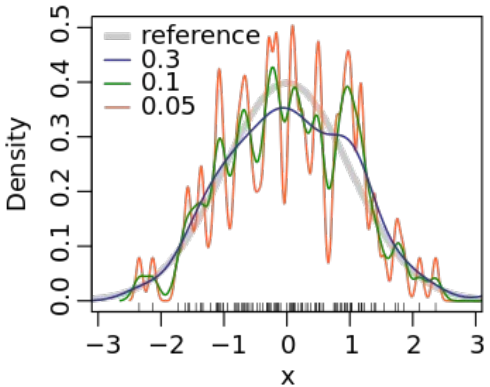
\includegraphics[width=0.4\linewidth]{images/chapter_2/Bandwidth.png}
    \caption{KDE Bandwidth}
\end{figure}

To summarize, compared to a histogram, KDE produces plots that are much less cluttered and highly interpretable. However, it suffers from potential distortions if the underlying distribution has hard boundaries or lacks smoothness, and its accuracy heavily depends on selecting the appropriate smoothing parameter (bandwidth).

\subsection{CDF: Cumulative Distribution Function}
The Cumulative Distribution Function (CDF) is a function of $x$, where $x$ represents any value that might appear within a given distribution. 

Probability that a random variable $X$ will take a value less than or equal to a specific value $x$, :
$$F_X(x) := P(X \le x)$$

Also used to calculate the probability that a value falls within a specific interval between $a$ and $b$:
$$P(a \le X \le b) = F_X(b) - F_X(a)$$

The CDF provides a clear visual representation of the distribution's overall shape. Highly probable values and common intervals appear as steep, nearly vertical sections on the CDF graph, indicating a high concentration of data points in that specific range. Conversely, flat sections indicate ranges with very few data points.

\begin{figure}[h]
    \centering
    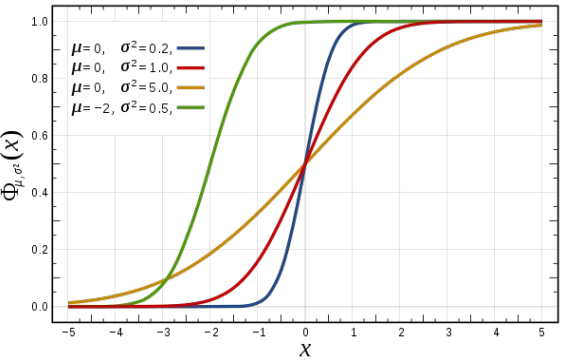
\includegraphics[width=0.4\linewidth]{images/chapter_2/CDF_Example.png}
    \caption{CDF}
\end{figure}

\subsection{ECDF: Empirical Cumulative Distribution Function}
The Empirical Cumulative Distribution Function (ECDF) is an estimate of the CDF that generated the points in the sample. To evaluate ECDF($x$) for a particulare value of $x$, it is needed to compute the fraction of values in the distribution less than or equal to $x$. ECDF is a step function that jumps up by $1/m$ at each of the $m$ data points. It's a really good estimation of the CDF, even if it's a step function.

\subsection{Percentiles}
Percentile indicates the value below which a given percentage of observations in a group of observation falls. Representing a feature through percentiles allow representing its entire distribution. The most famous percentiles are the quartiles $25^{th}$, $50^{th}$, and $75^{th}$.It is useful to remember than the $50^{th}$ represents the median, as 50\% of the values are smaller than it and the remaining 50\% are bigger. It is the mean only for the Gaussian Distribution. Finally, the outliers are easily found as for example they can be the values in the first and last percentile of the distribution.

\begin{figure}[h]
    \centering
    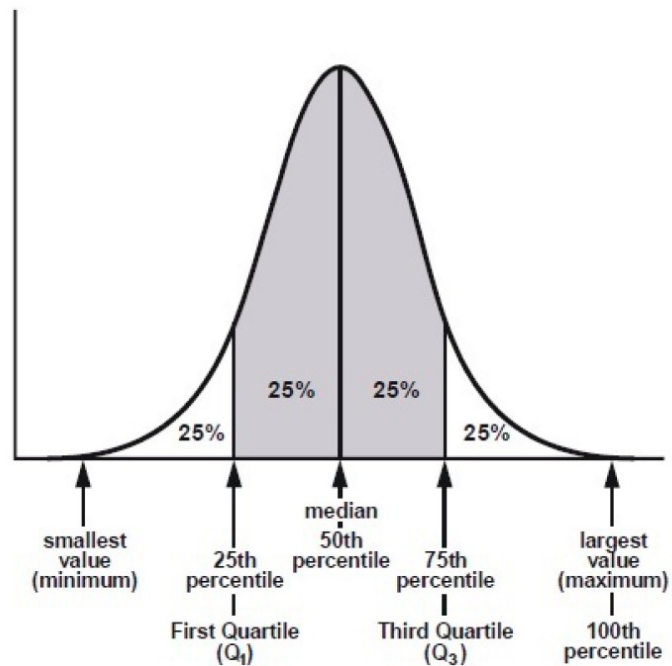
\includegraphics[width=0.5\linewidth]{images/chapter_2/Percentile.png}
\end{figure}

\subsection{Boxplot}
Boxplots are a standardized way of displaying the distribution of data based on summary values:


\begin{itemize}
    \item \textbf{Median:} $50^{th}$ percentile ($Q2$) the middle value of the attribute, not the mean.
    \item \textbf{First Quartile:} middle number between the smallest number excluding outliers (not minimum) and the median of the attribute.
    \item \textbf{Third Quartile:} the middle value between the median and the highest value excluding outliers (not the maximum) of the attribute.
    \item \textbf{Interquatile Range (IQR):} $25^{th}$ to the $75^{th}$ percentile.
    \item \textbf{Whiskers:} lines that exit from the boxplot (shown in blue).
    \item \textbf{Outliers:} samples (points) that fall outside of the range: $(Q1 - (1.5 * IQR)) \rightarrow (Q3 + (1.5 * IQR))$
\end{itemize}

\begin{figure}[h]
    \centering
    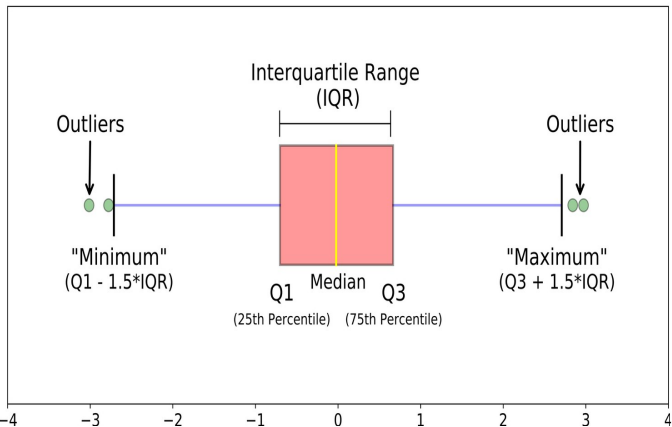
\includegraphics[width=0.4\linewidth]{images/chapter_2/Boxplot.png}
\end{figure}

It is important to know that box plot won't be symmetrical if the underlying distribution is not a Gaussian distribution.

\begin{figure}[h]
    \centering
    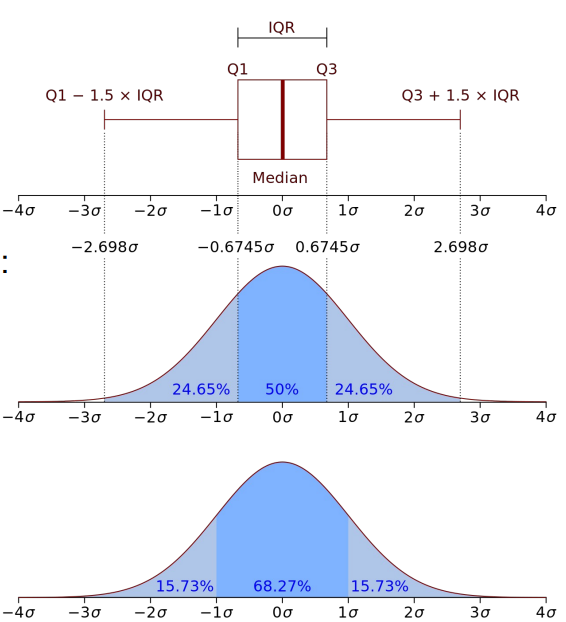
\includegraphics[width=0.4\linewidth]{images/chapter_2/Boxplot Example.png}
\end{figure}

\subsection{Outliers}
Outliers are extreme values that might be errors in measurement and recording or rather accurate reports of rare events. The best way to define and handle outliers depends on domain knowledge, such as information about where the data come from, what they mean and the scope of the analysis.Outliers can be detected through univariate analysis (boxplots, percentiles, GESD) or multivariate analysis (DBSCAN).

\begin{itemize}
    \item \textbf{GESD:} Generalized Extreme Studentized Deviate is used to detect one or more outliers in a univariate dataset that follows a normal distirbution. The GESD test performs separate tests for 1 outlier up to an upper bound $k$ of outliers, where a test statistic $R$ is recomputed recursively up to the $k$-th outlier.
    \item \textbf{DBSCAN:} is density based clustering non parametric algorithm used in multivariate analysis, as it groups together points that are closely packed together (points with many nearby neighbors), while marking as outliers points that lie alone in low density regions, whose nearest neighbors are too far away.
\end{itemize}

\begin{figure}[h]
    \centering
    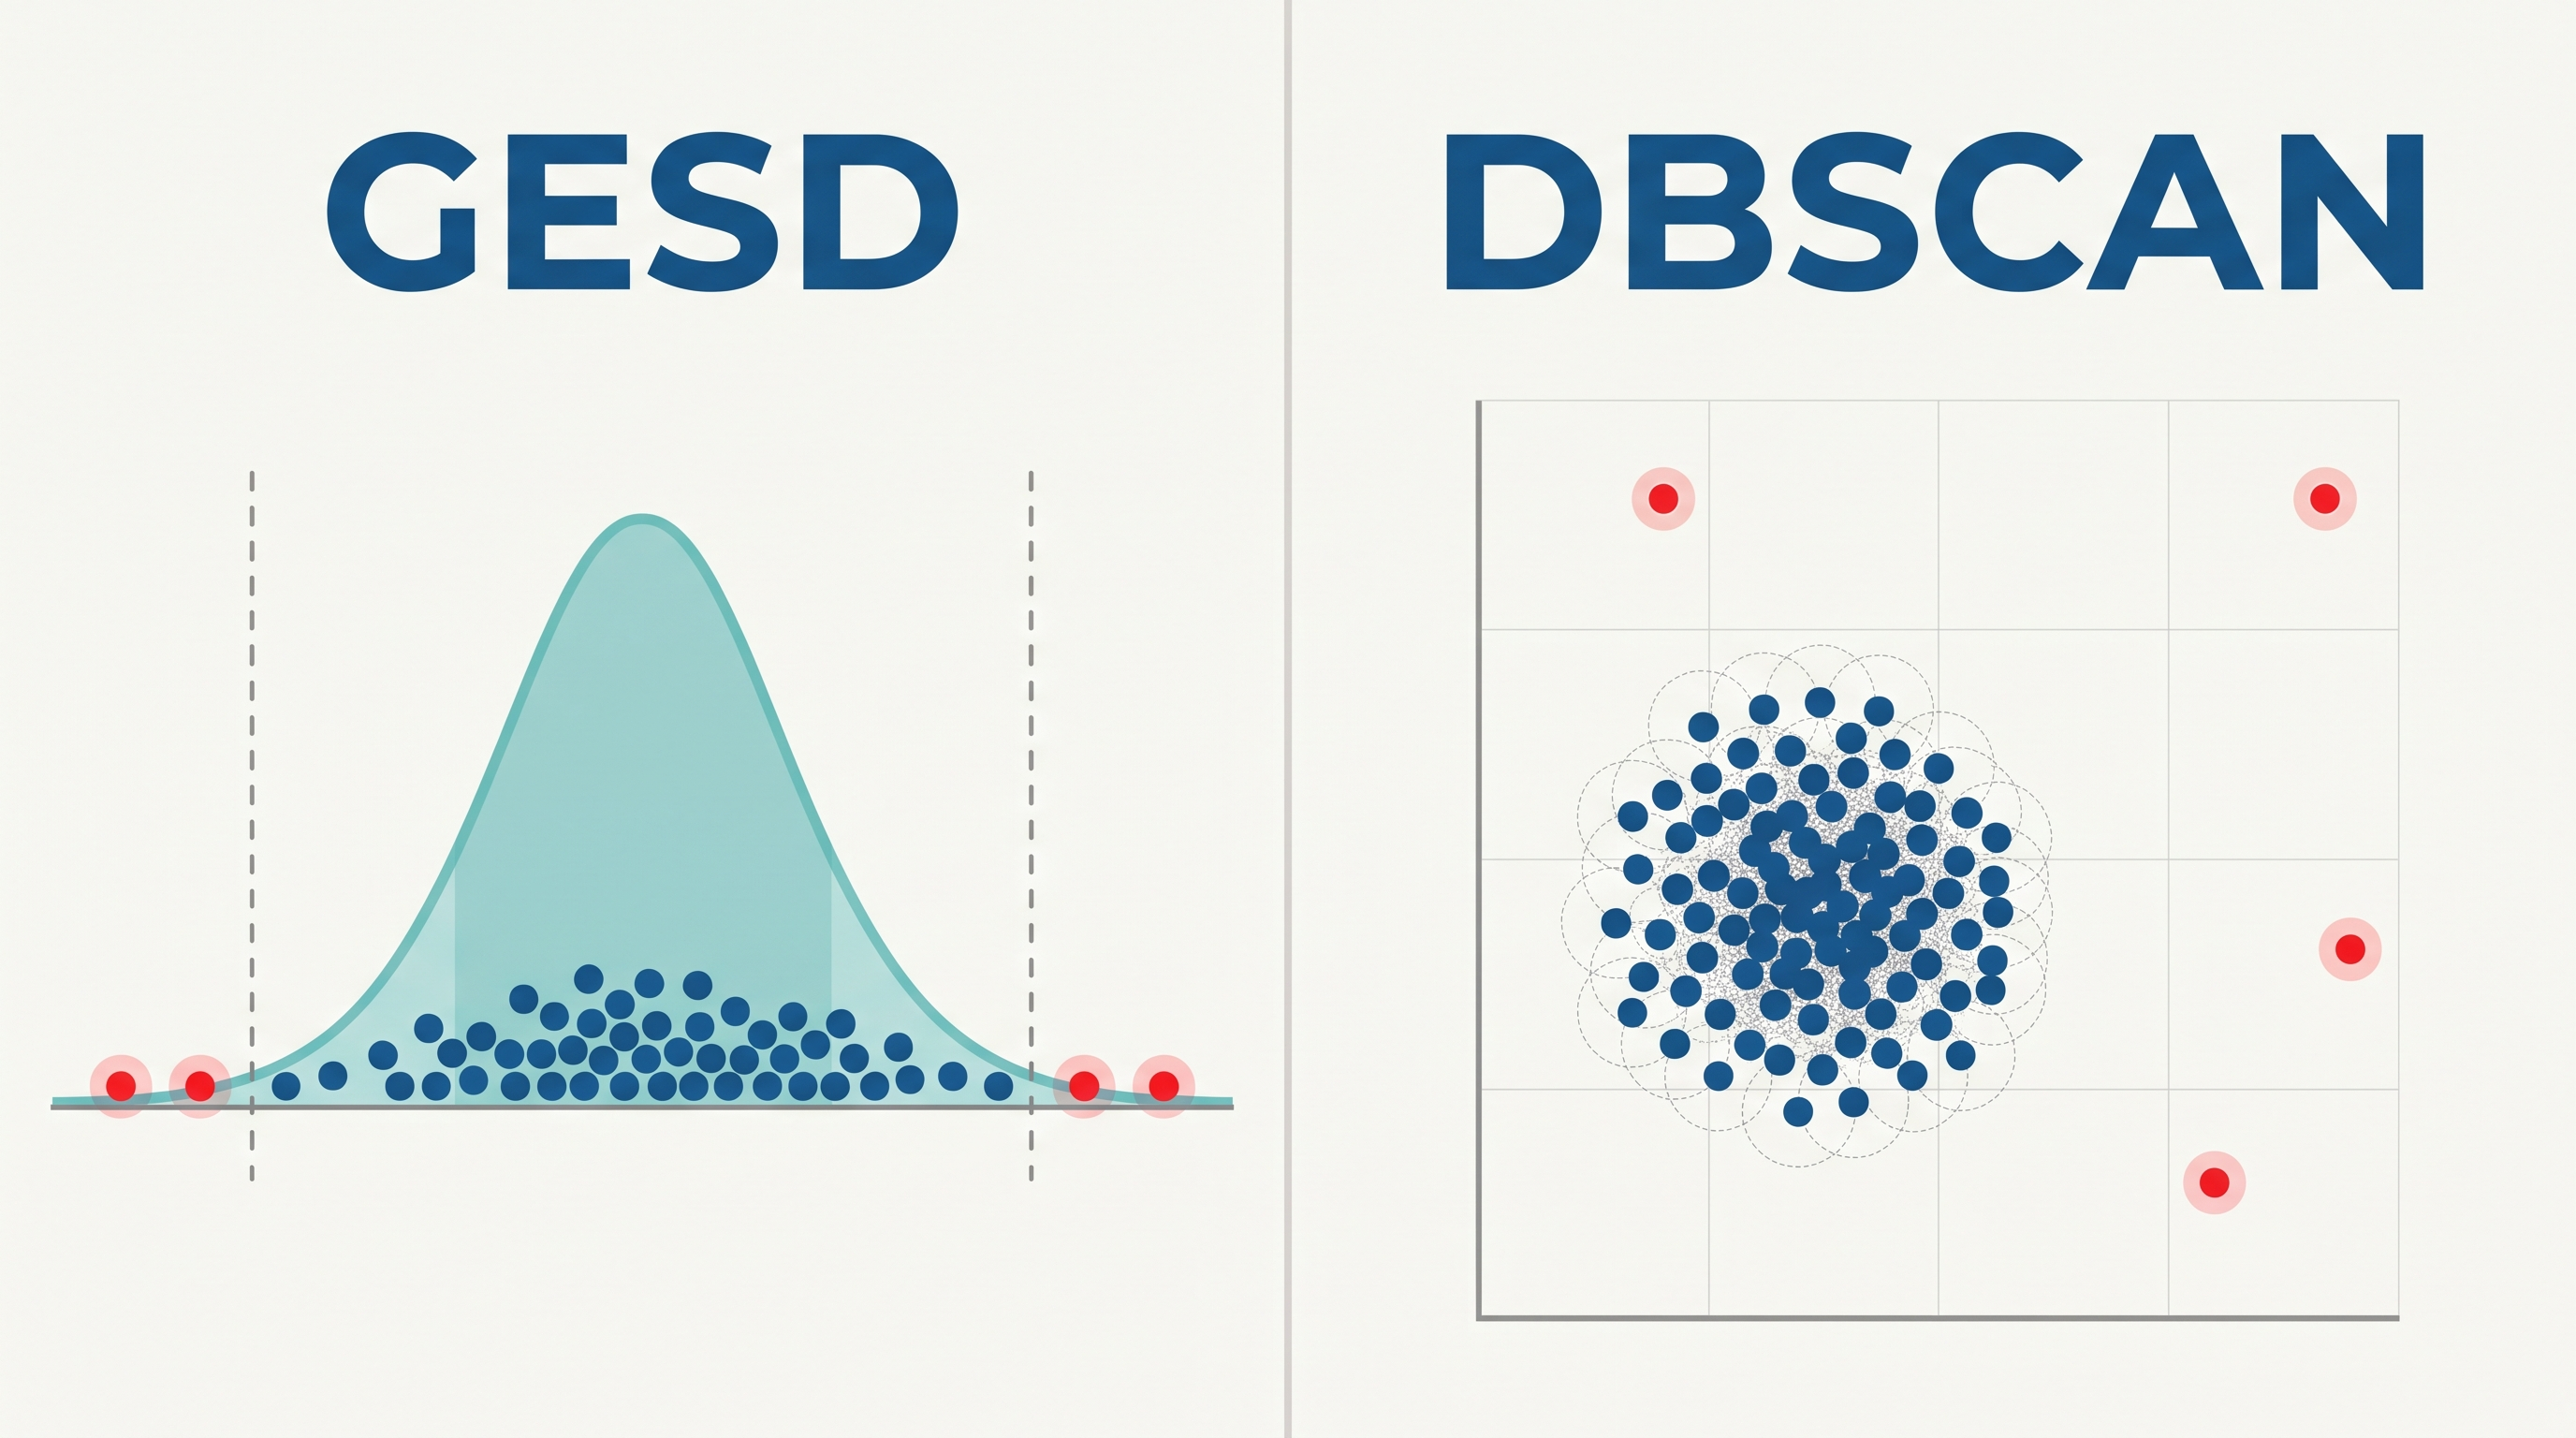
\includegraphics[width=0.4\linewidth]{images/chapter_2/GESD_DBSCAN.png}
\end{figure}

\section{Correlation Analysis}
Datasets usually include different features and the description of the main relations, namely the correlation, between different features assumes a key role.The correlation is the measure of the relationship between two data objects and it is useful during the data exploration phase in order to perform analysis of feature correlation.

\subsection{Scatter Plot}
Scatter plots are the simplest way to visually check for a relationship between 2 variables, but they don't allow you to see if there are many points in the same position or just one, since the data are affected by rounding and conversion. A possible solution to this issue is to jitter the data by adding noise to reverse the effect of rounding off. 

\begin{figure}[h]
    \centering
    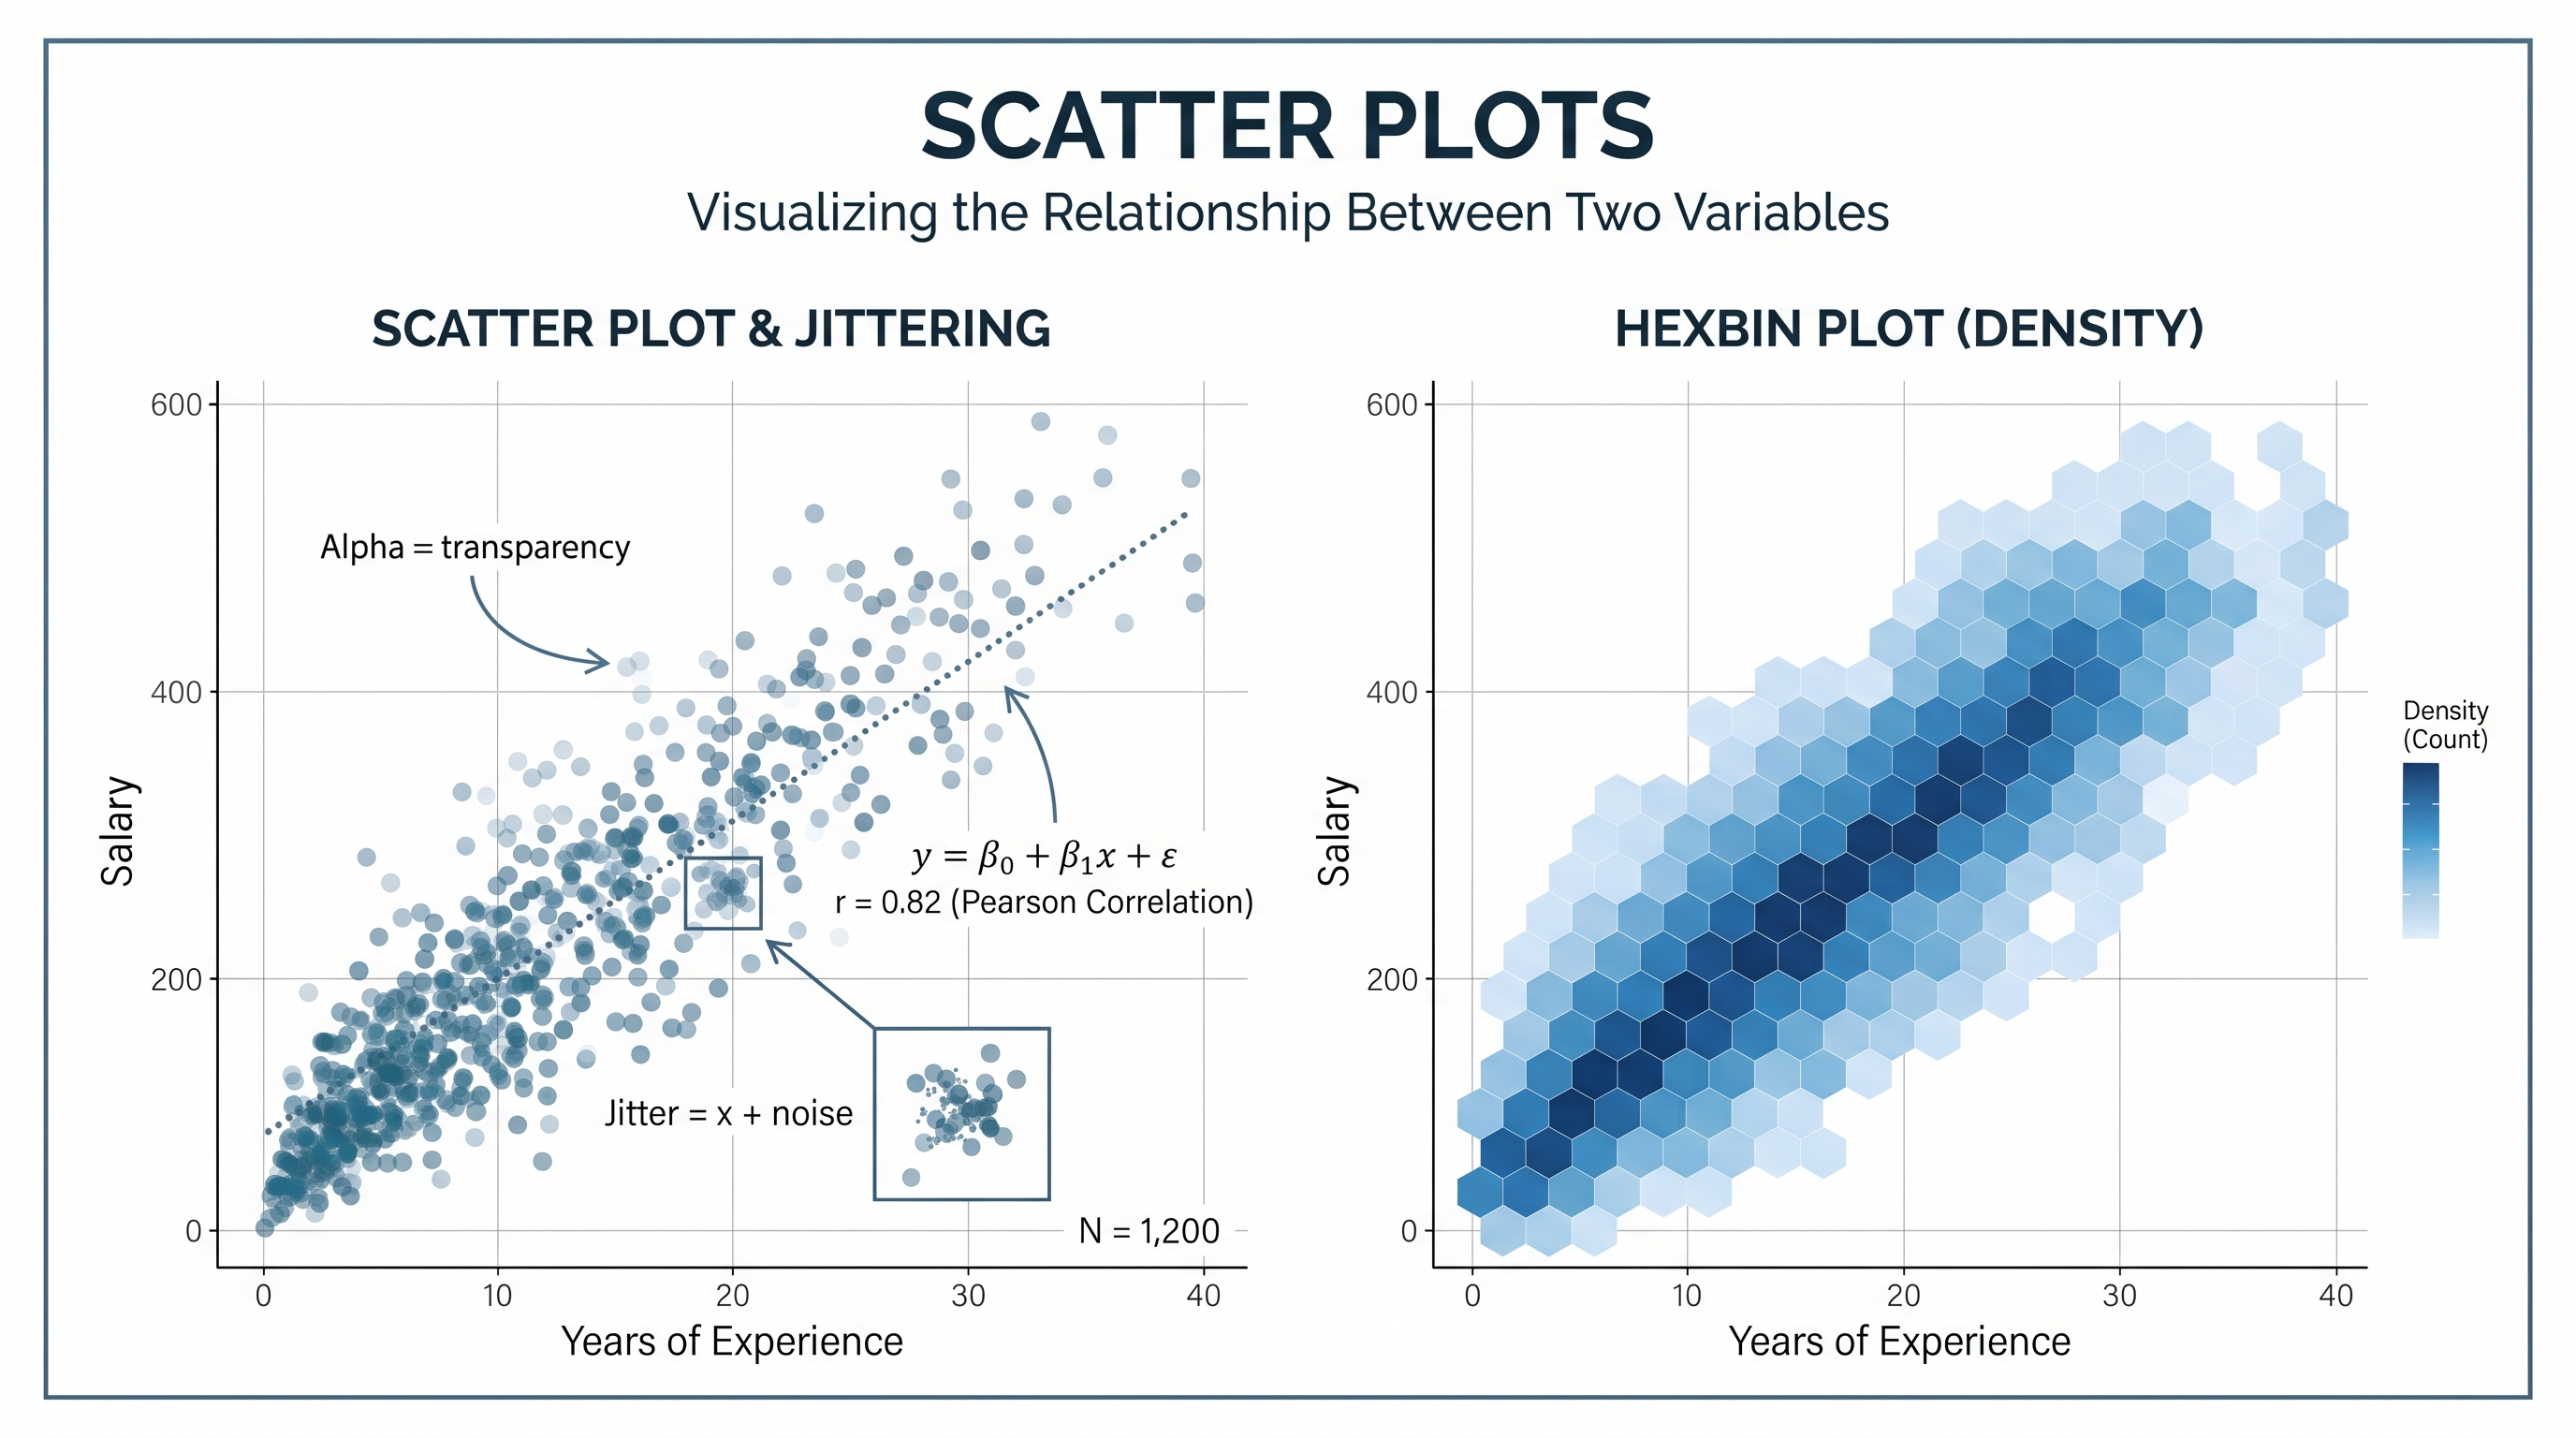
\includegraphics[width=0.35\linewidth]{images/chapter_2/Scatter.png}
    \caption{Scatter Plot}
\end{figure}

Then adding an alpha parameter (transparency) to each point in order to retrieve density information, where darker zones correspond to higher density zones. There is also the possibility to build hexbin plots and scatter plot percentiles, where it is required to bin one variable and plot a curve for the two variables in each bin.Moreover, Correlation is a statistic quantity indented to quantify the strength of the relationship between 2 variables. There are different ways to compute correlations:

\begin{itemize}
    \item \textbf{Covariance:} in order to compare two variables they must have same unit of measurement or alternatively be normalised.
    \item \textbf{Pearson's Correlation} is a single number that states how much 2 features are meanly correlated, if -1 negatively correlated, if 1 perfectly positively correlated. 0 for not linear correlated. Pearson's Correlation solves the problem of normalization, needed by the Covariance, but it only detects linear correlation, so for instance it is unable to detect quadratic correlation, and all the other non-linear correlations.
\end{itemize}

\begin{figure}[h]
    \centering
    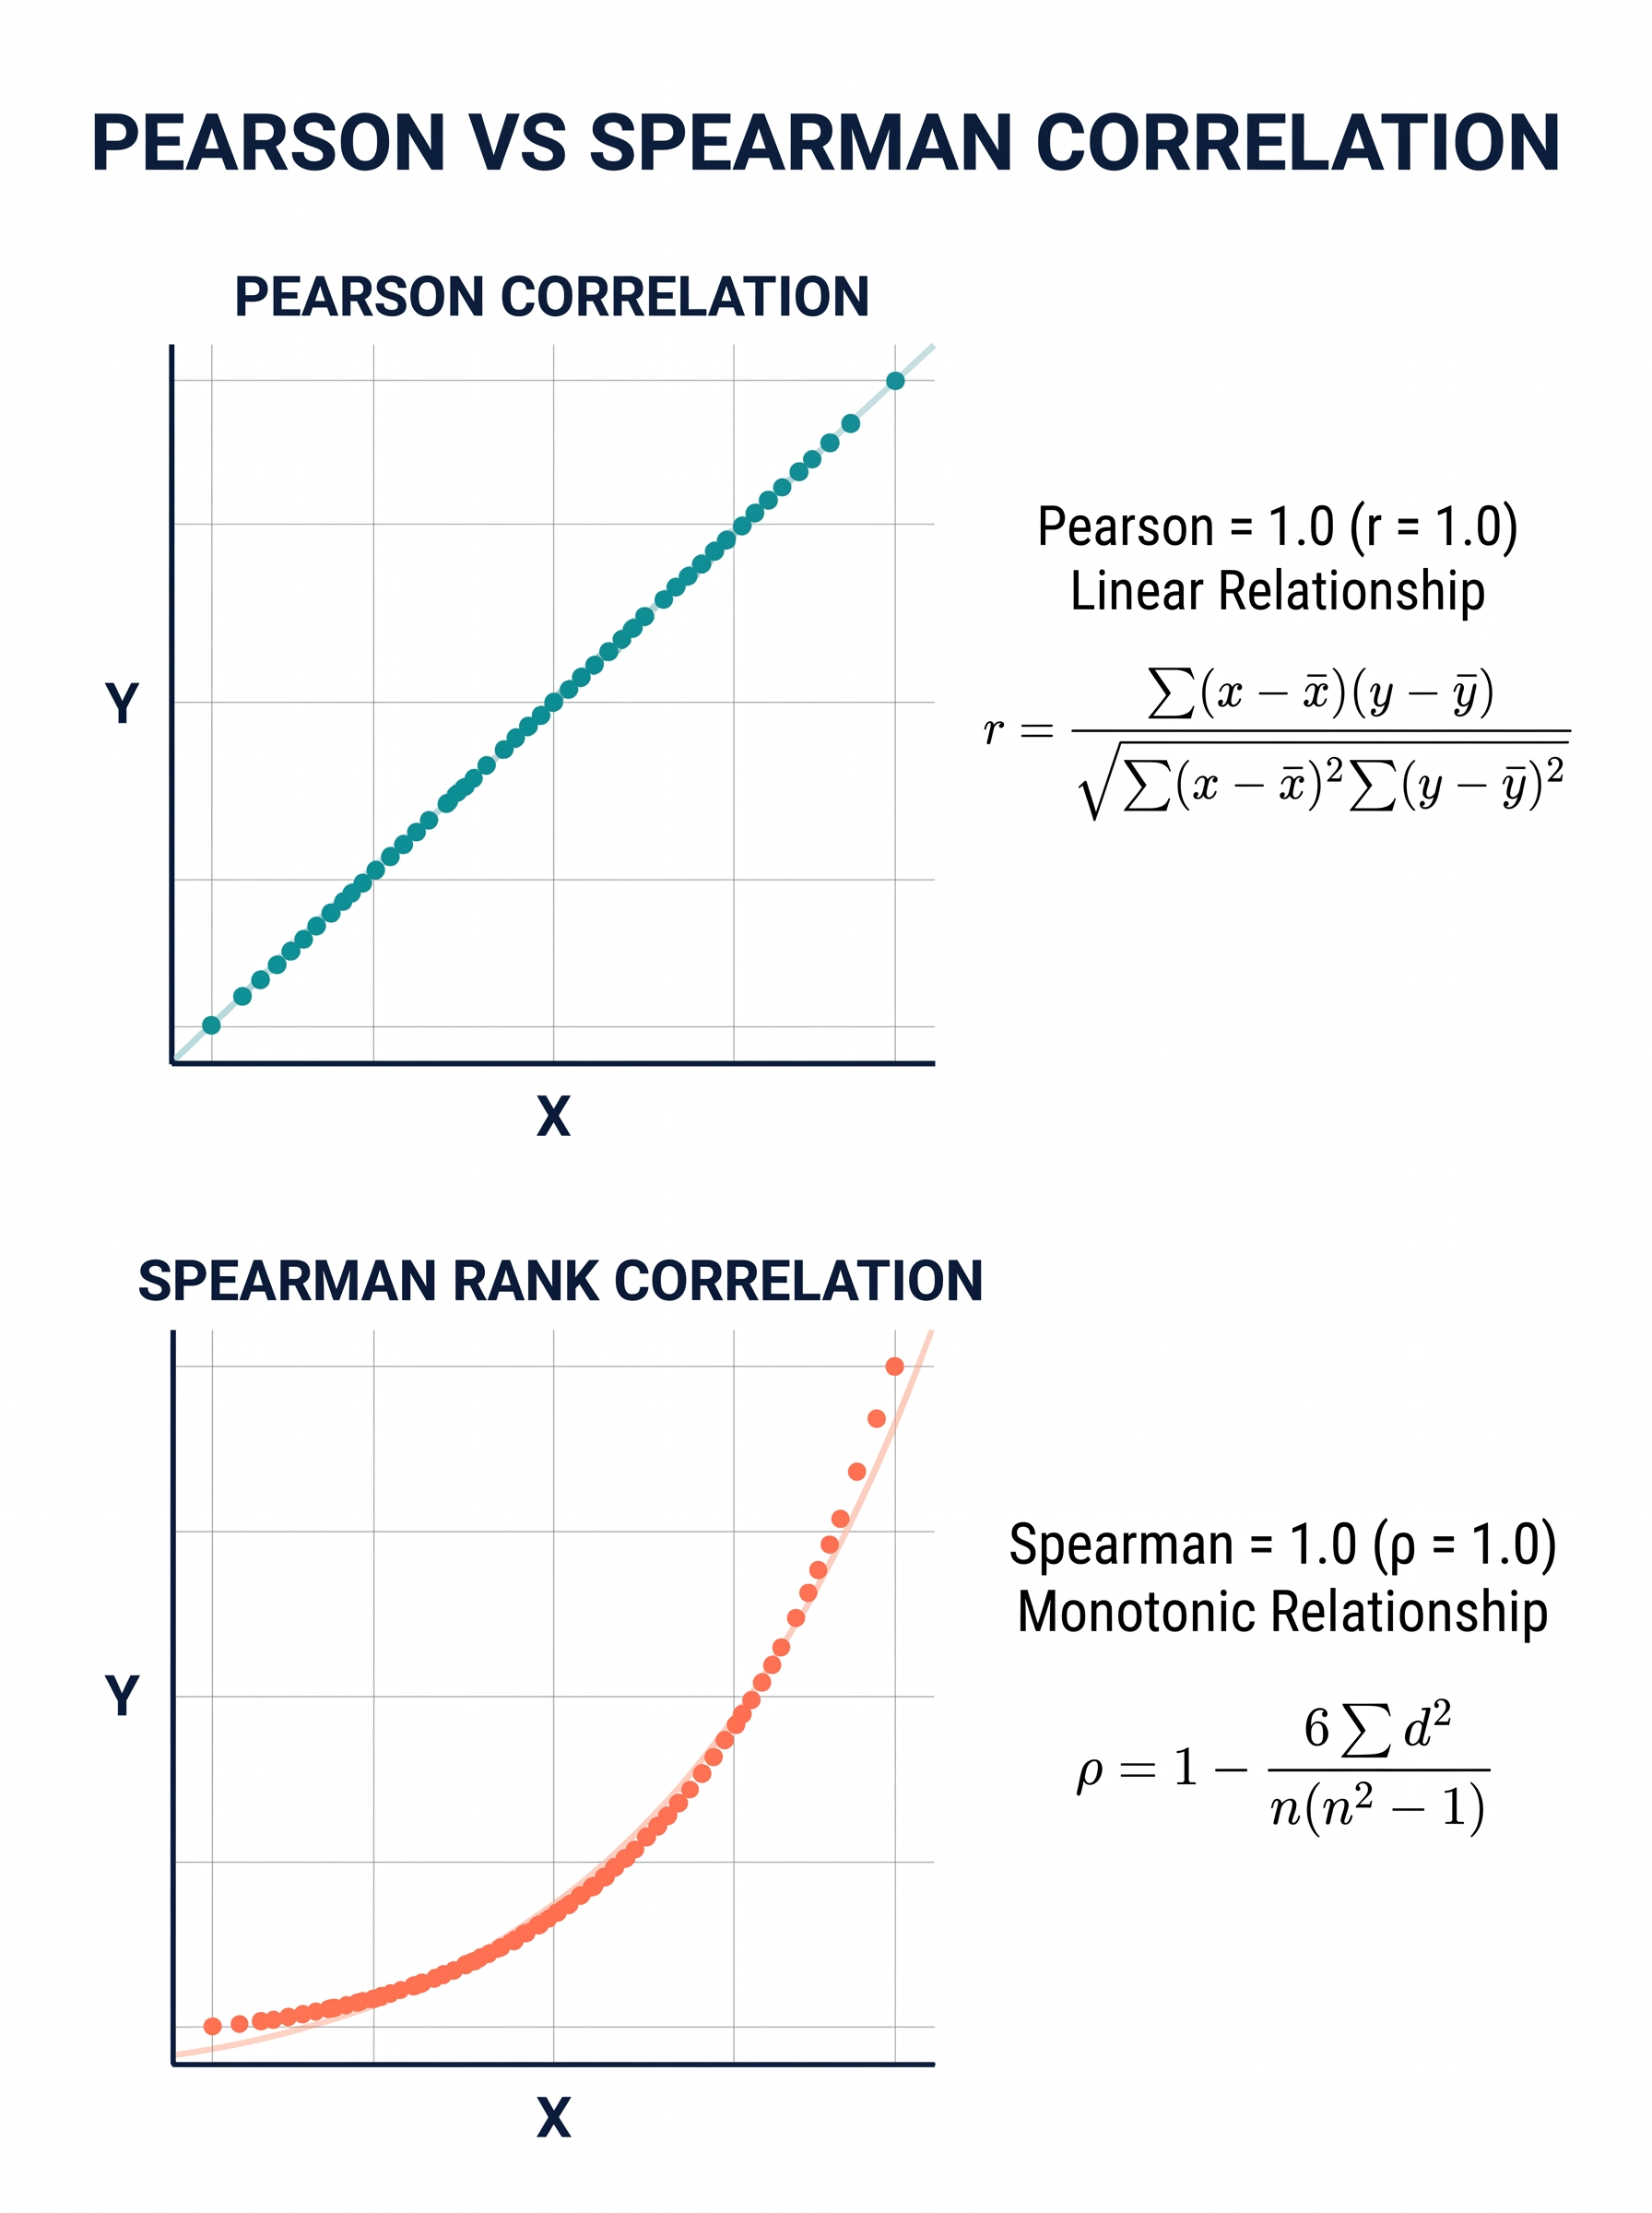
\includegraphics[width=0.35\linewidth]{images/chapter_2/Pearson_Spearman.png}
    \caption{Pearson and Spearman Correlation}
\end{figure}

\begin{figure}[h]
    \centering
    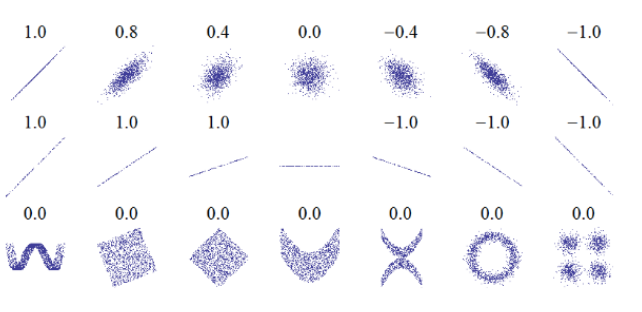
\includegraphics[width=0.35\linewidth]{images/chapter_2/Pearson_non_Linear_correlation.png}
    \caption{Pearson Non Linear Correlation}
\end{figure}

In addition, there are some types of nonlinear correlations that Pearson's correlation can't detect, such as perfectly horizontal, if one variable is always constant the formula doesn't detect it.

\begin{itemize}
    \item \textbf{Spearman's Rank Correlation:} Spearman index uses the variables rank instead of Pearson that used the variables themselves. It assesses how well the relationship between 2 variables can be described using a monotonic function. In some cases the Spearman index saves from some corner cases of Pearson index returning a value close to 0. The method for applying it is the following:
    \begin{itemize}
        \item Rank the 2 dataset, ranking is achieved by giving the ranking 1 to the biggest number in a column, 2 to the second biggest one and so on. The smallest value in the column will get the lowest ranking.
        \item If using the simplified rank formula: Indicate $m$ as the number of different ranks.
        \item Tied scores are given the mean (average) rank. For example, if there are 3 tied scores ranked $5^{th}$ ($5^{th}$, $6^{th}$, $7^{th}$) the mean rank is calculated as $(5+6+7)/3 = 6$.
        \item Find the difference in the ranks, that is the difference between the ranks of the two values on each row.
        \item Compute the formula, either in the general case or in the integer simplified case.
    \end{itemize}
\end{itemize}

\textbf{Spearman's Rank Correlation Example:} $X = (3,0,1)$, $Y = (-1,50,2)$
\begin{enumerate}
    \item rank both datasets: $X=(1,3,2)$ $Y=(3,1,2)$
    \item indicate $m$ as the number of different ranks, in this case $m = 3$
    \item compute the difference $X_i - Y_i$: $(-2,2,0)$
    \item use the formula, in this case the simplified integer ranks formula: $r_s = 1 - (6 * (4 + 4))/(3 - 8) = -1$
\end{enumerate}

\begin{figure}[h]
    \centering
    \includegraphics[width=0.35\linewidth]{images/chapter_2/chapter_2/Spearman_Rank_Examples.png}
\end{figure}

In addition Spearman's rank is 1 when both variable are correlated by an increasing monotonic function, while -1 if the function is decreasing monotonic. 0 if there isn't a monotonic function correlation. To sum up, Spearman's rank detects monotonic correlation between 2 variables, not only linear correlation as Pearson does.

\section{Data Visualization: Advanced Techniques}

\subsection{Heatmap}
A heatmap is a colorful grid that makes it easy to read a correlation matrix. Instead of looking at raw numbers to see how strongly two variables are linked, you look at colors. For example, a dark red square might mean a strong positive relationship, while a dark blue one means a strong negative relationship. The grid is perfectly symmetric: the relationship between variable A and variable B is the exact same as the relationship between B and A.

\begin{figure}[h]
    \centering
    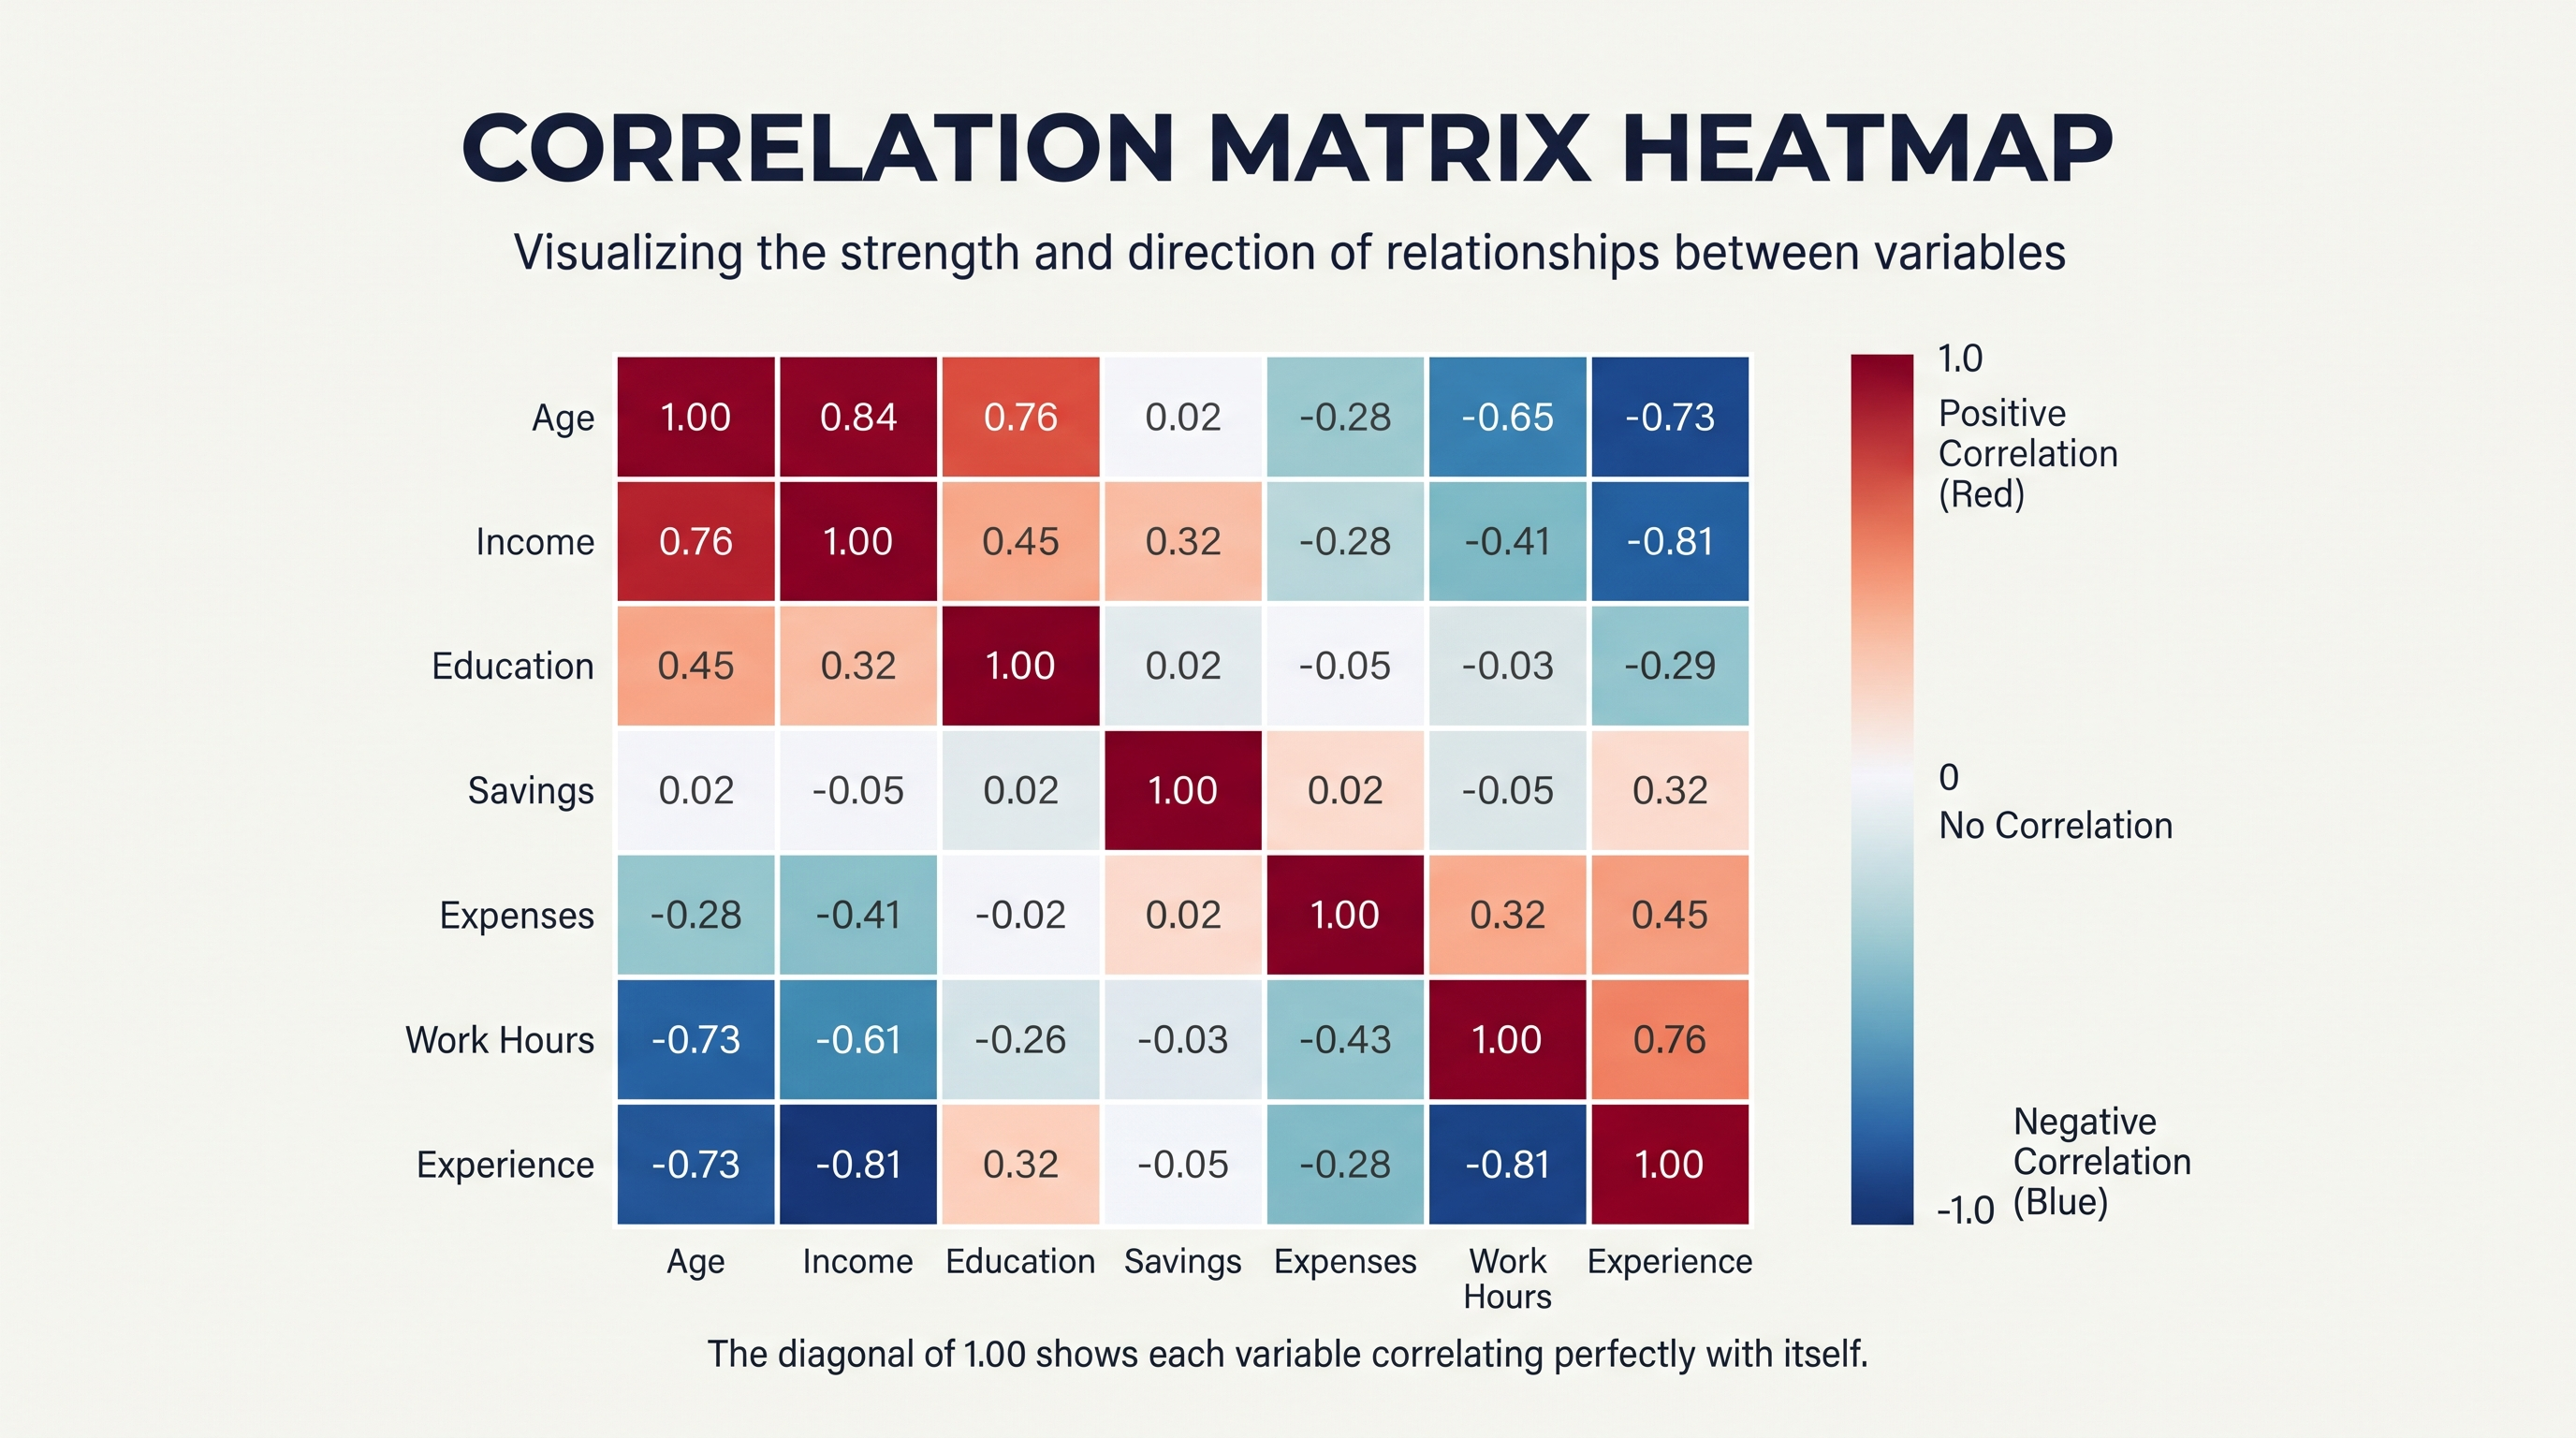
\includegraphics[width=0.5\linewidth]{images/chapter_2/Heatmap.png}
\end{figure}

\subsection{Dimensionality Reduction: PCA and t-SNE}
When a dataset has dozens or hundreds of features, plotting it on a standard 2D graph is impossible. To fix this, we use mathematical techniques to compress the dataset into just 2 or 3 new features without losing too much important information. 

\begin{figure}[h]
    \centering
    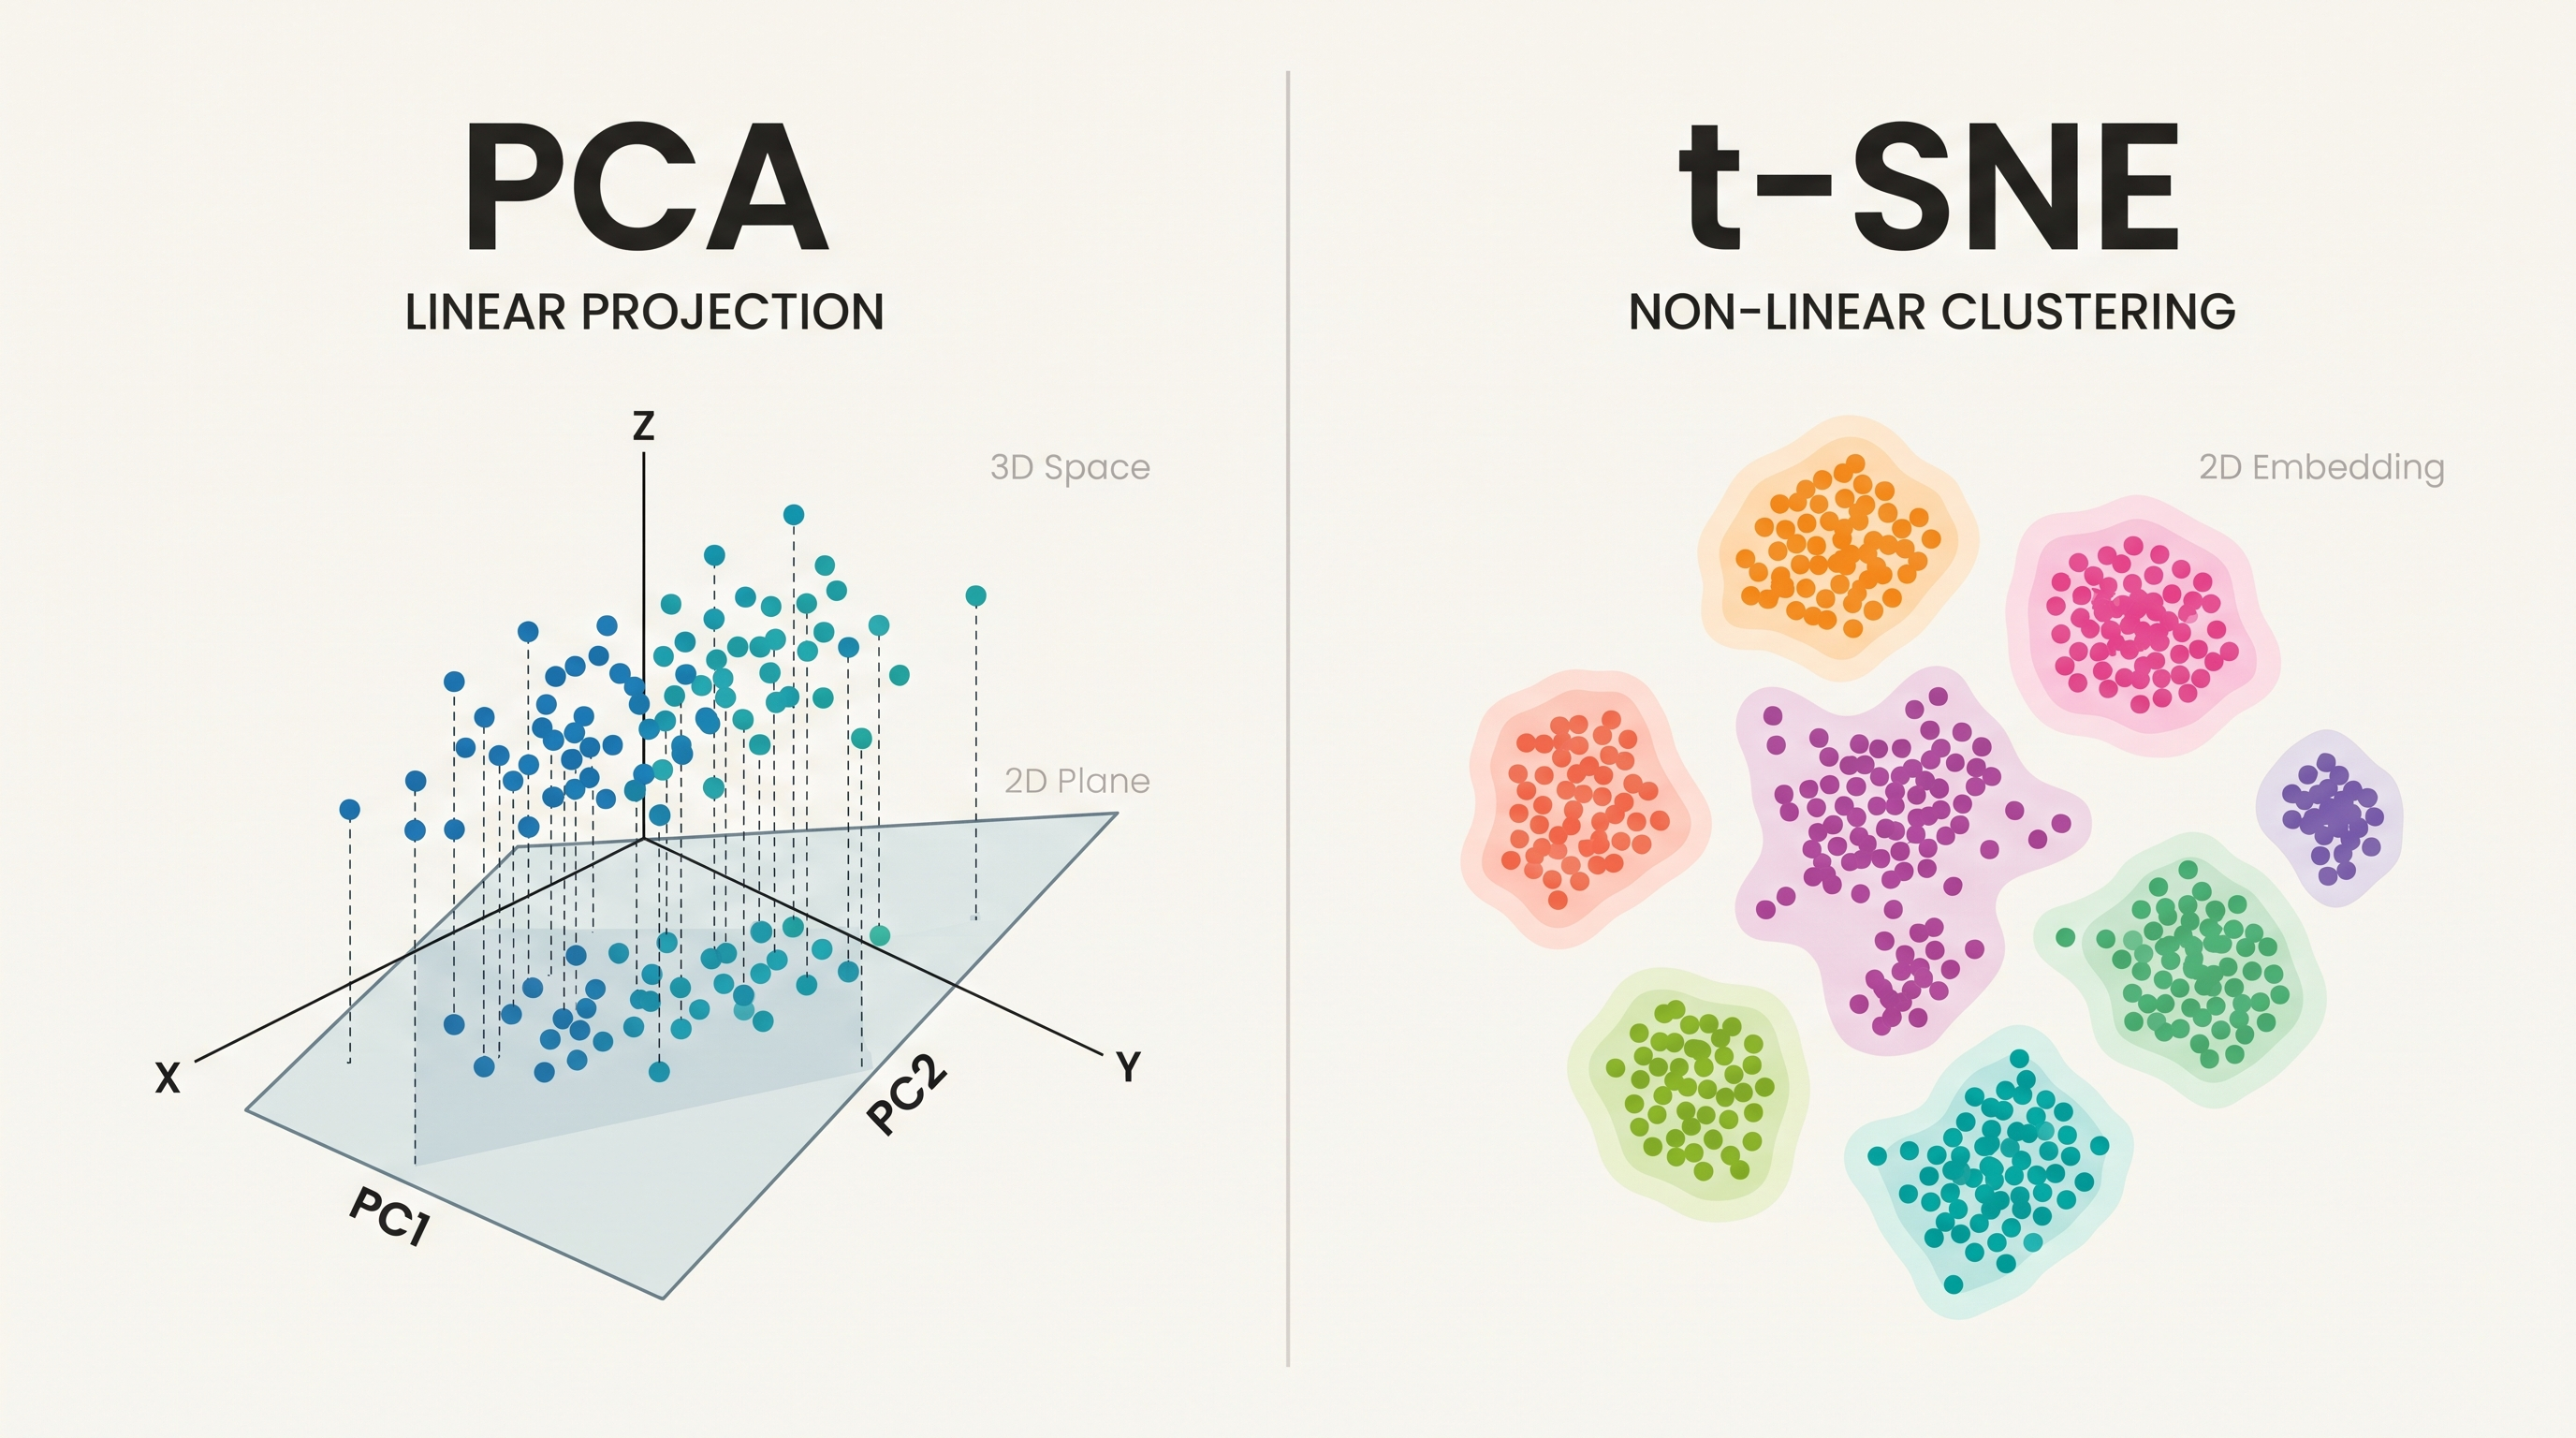
\includegraphics[width=0.5\linewidth]{images/chapter_2/PCA_tSNE.png}
\end{figure}

\begin{itemize}
    \item \textbf{PCA (Principal Component Analysis):} This method shrinks the data by finding the main linear directions that contain the most information. It provides a broad, global overview of the dataset's general trends.
    \item \textbf{t-SNE (t-Distributed Stochastic Neighbor Embedding):} This is a more complex, non-linear technique. It focuses on keeping similar data points close to each other, making it excellent for spotting distinct groups or clusters on a 2D map.
\end{itemize}

Visualizing data is crucial for understanding it, but picking the right chart or reduction method depends entirely on what underlying patterns you want to discover.


\section{A prova di coglione}

\paragraph*{Il dataset.}
Tabella di $M$ righe (istanze, record, oggetti, campioni) e $N$ colonne (attributi, feature). Le sue dimensioni condizionano l'analisi, perché alcuni algoritmi richiedono molte risorse hardware su dataset grandi. Si riducono con il \textbf{data sampling} (meno righe, $m'<m$) o con la \textbf{feature selection} (meno colonne, $n'<n$). L'esplorazione può essere \textbf{univariata} (una colonna alla volta) o \textbf{multivariata} (relazioni tra più colonne). Per ogni attributo servono unità di misura, tipo (categorico o numerico) e dominio, verificando che i valori rispettino i vincoli del dominio. Notazione usata: $a\in\mathcal A$ (appartenenza), $|\mathcal A|$ (cardinalità), $\subseteq$ e $\subset$ (sottoinsieme e sottoinsieme stretto), $\mathbb N$, $\mathbb R$, $\{0,1\}$, $[0,1]$, vettore $\mathbf x=(x_1,\dots,x_n)^T$ e norma $\|\mathbf x\|$ (di solito euclidea).

\subsection*{Analisi univariata: la distribuzione}

Una feature è una \textbf{variabile aleatoria} $X$ e i dati raccolti $x_1,\dots,x_m$ sono le sue realizzazioni. La legge che li ha generati (\textbf{distribuzione teorica}) è ignota, quindi ci si affida alla \textbf{distribuzione empirica}, di solito visualizzata con un \textbf{istogramma}: l'intervallo dei dati è diviso in \emph{bin} consecutivi e se ne conta la frequenza. Le distribuzioni sono \textbf{discrete} (descritte da una funzione di massa, PMF) o \textbf{continue} (descritte da una funzione di densità, PDF, come la gaussiana). Con molti campioni la PMF è illeggibile: si ricorre alla CDF o al confronto tra distribuzioni.

\paragraph*{KDE (Kernel Density Estimation).}
Stima la PDF dai campioni ed è una versione \emph{liscia e continua} dell'istogramma. Calcola la densità come media pesata dei punti vicini, con pesi dati da un \textbf{kernel} $K$ (tipicamente gaussiano) più alti per i punti più prossimi:
$$\hat f_h(x)=\frac{1}{mh}\sum_{i=1}^m K\!\left(\frac{x-x_i}{h}\right)$$
La \textbf{bandwidth} $h$ controlla la levigatezza. Se è troppo grande (\emph{over-smoothing}) cancella caratteristiche reali, se è troppo piccola (\emph{under-smoothing}) crea caratteristiche false dovute al rumore. Rispetto all'istogramma il grafico è più pulito e leggibile, ma si distorce con distribuzioni dai bordi netti o non lisce e dipende dalla scelta di $h$.

\paragraph*{CDF ed ECDF.}
La \textbf{CDF} $F_X(x)=P(X\le x)$ dà la probabilità di restare sotto $x$, e $P(a\le X\le b)=F_X(b)-F_X(a)$. I tratti ripidi indicano valori frequenti, quelli piatti zone quasi vuote. L'\textbf{ECDF} la stima dai campioni: è la frazione di valori $\le x$, una funzione a gradini che sale di $1/m$ a ogni dato, ma approssima molto bene la CDF.

\paragraph*{Percentili e boxplot.}
Il \textbf{percentile} è il valore sotto cui cade una data percentuale delle osservazioni, quindi i percentili descrivono l'intera distribuzione. I più usati sono i quartili (25°, 50°, 75°); il 50° è la \textbf{mediana}, che coincide con la media solo nella gaussiana. Il \textbf{boxplot} riassume la distribuzione con: mediana ($Q2$), $Q1$ e $Q3$ (calcolati escludendo gli outlier), \textbf{IQR} (da $Q1$ a $Q3$), \emph{whiskers} (i baffi) e \textbf{outlier}, i punti fuori da $[\,Q1-1.5\,\mathrm{IQR},\;Q3+1.5\,\mathrm{IQR}\,]$. Se la distribuzione non è gaussiana, il boxplot non è simmetrico.

\paragraph*{Outlier.}
Valori estremi che possono essere errori di misura o registrazione, oppure segnalazioni corrette di eventi rari: come trattarli dipende dalla conoscenza del dominio (origine dei dati, significato, scopo dell'analisi). Si rilevano con metodi univariati (boxplot, percentili, GESD) o multivariati (DBSCAN):
\begin{itemize}
    \item \textbf{GESD}: test per trovare uno o più outlier in un dataset univariato \emph{normale}; ripete i test da 1 fino a un massimo di $k$ outlier, ricalcolando la statistica $R$.
    \item \textbf{DBSCAN}: clustering non parametrico basato sulla densità; raggruppa i punti molto vicini e segna come outlier quelli isolati in zone a bassa densità, con vicini troppo lontani.
\end{itemize}

\subsection*{Analisi di correlazione}

La \textbf{correlazione} misura la relazione tra due variabili e guida l'esplorazione delle feature.

\paragraph*{Scatter plot.}
È il modo più semplice per vedere una relazione tra due variabili, ma arrotondamenti e conversioni sovrappongono i punti, nascondendone la densità. Si rimedia con il \textbf{jitter} (rumore che annulla l'effetto dell'arrotondamento), con la \textbf{trasparenza} $\alpha$ (zone scure = alta densità), con gli \textbf{hexbin} o con gli \textbf{scatter plot a percentili} (una variabile divisa in bin, con una curva per ciascun bin).

\paragraph*{Indici di correlazione.}
\begin{itemize}
    \item \textbf{Covarianza}: confronta due variabili solo se hanno la stessa unità di misura o sono normalizzate.
    \item \textbf{Pearson}: un solo numero che risolve la normalizzazione, $-1$ per correlazione negativa perfetta, $+1$ per positiva perfetta, $0$ per assenza di correlazione \emph{lineare}. Vede solo relazioni lineari: non coglie quelle quadratiche o non lineari in genere, né il caso di una variabile costante.
    \item \textbf{Spearman}: usa i \emph{ranghi} invece dei valori e misura quanto la relazione sia descrivibile da una funzione \textbf{monotona}. Vale $1$ se la funzione è crescente, $-1$ se decrescente, $0$ se non c'è monotonia. Evita alcuni casi limite in cui Pearson dà valori vicini a 0.
\end{itemize}

\textbf{Calcolo di Spearman.} Si assegnano i ranghi a ogni colonna (1 al valore maggiore, e così via; i pari merito ricevono il rango medio, ad esempio tre valori al 5°, 6°, 7° posto ricevono $(5+6+7)/3=6$), si calcolano le differenze $d_i$ tra i ranghi di ogni riga e si applica, per ranghi interi e $m$ ranghi distinti,
$$r_s=1-\frac{6\sum_i d_i^2}{m(m^2-1)}$$
\emph{Esempio}: $X=(3,0,1)$ e $Y=(-1,50,2)$ hanno ranghi $(1,3,2)$ e $(3,1,2)$, quindi $d=(-2,2,0)$ e $r_s=1-\frac{6\cdot 8}{3\cdot 8}=-1$ (relazione monotona decrescente).

\subsection*{Visualizzazione avanzata}

\begin{itemize}
    \item \textbf{Heatmap}: griglia colorata che rende leggibile una matrice di correlazione al posto dei numeri (rosso scuro = correlazione positiva forte, blu scuro = negativa forte). È simmetrica, perché la relazione A–B coincide con quella B–A.
    \item \textbf{Riduzione di dimensionalità}: con decine o centinaia di feature non si può tracciare un grafico 2D, quindi si comprime il dataset in 2 o 3 nuove feature perdendo poca informazione. \textbf{PCA} trova le direzioni lineari principali che contengono più informazione e dà una visione globale delle tendenze. \textbf{t-SNE} è non lineare e mantiene vicini i punti simili, ottimo per individuare gruppi e cluster.
\end{itemize}

Visualizzare è fondamentale per capire i dati, ma il grafico o la riduzione giusti dipendono dai pattern che si vogliono scoprire.